% \published{statement_of_authorship.jpg}
\chapter{ Description of the model \label{ch:numero_uno}}
\section{An invitation to implicit curve modeling}
To motivate the primary mechanism by which cells will undergo mitosis in this thesis, we consider a toy example in which the equations for two spheres undergo a catastrophic topological change as one parameter changes.

We start by considering the equations for two spheres which begin as coincident and move apart as the parameter $a$ becomes larger. In order to combine the first equation
\begin{equation*}
f_1(x,y,z) = R^2 - \left[ (z+a)^2+y^2+z^2 \right],
\end{equation*}
with the second equation
\begin{equation*}
f_2(x,y,z) = R^2 - \left[ (z-a)^2+y^2+z^2 \right],
\end{equation*}
we require a smooth combination function. We construct the combined implicit curve as
\begin{equation*}
f(x,y,z) = \frac{1}{k}\ln{ \left( e^{k f_1(x,y,z)}+ e^{k f_2(x,y,z)} \right) }.
\end{equation*}
As shown in Figure \ref{fig:ToyMitosis}, we have a smooth splitting of a cell as the parameter $a$ ranges from $0.0$ to $5.0$. Note that $R$ is the nominal sphere radii, and $k$ is a smoothing parameter. The smaller $k$ is, the more smoothly the two curves cling to each other. 

In order to visualize the curves, we plot the level-$0$ curve using MATLAB's \codeword{isosurface} function. As we will see, for the purpose of the thesis

\begin{figure}[h]
\centering
\includegraphics[width=1\textwidth]{chapter1/figures/CellDivisionDemo.pdf}
\caption{A toy example of mitosis using implicit equations for spheres in 3D. Stage 1 is $a= 0.0$, Stage 2 is $a= 1.67$, Stage 3 is $a=3.33$, Stage 4 is $a = 5.0$}
\label{fig:ToyMitosis}
\end{figure}
\filbreak

As will be discussed in the next section, for the purpose of this thesis, we will be modeling growing geometry using level ``sections" of implicit curves in 2D.

\section{Modeling growing geometry }
Cell colonies are modeled using level-sections of implicit curves in two dimensions. For example, a circle can be modeled as the level-0 set of the following equation
\begin{equation*}
    f(x,y) =R^2-( x^2 + y^2),
\end{equation*}
where $R$ is the radius of the circle. If the filled in circle, the disk, is required, then producing a surf plot of the function in the region where $f(x,y) \geq 0$ is sufficient. This can be achieved by modifying the value of $f(x,y)$ to be \codeword{nan} wherever $f(x,y)<0$ so that MATLAB's \codeword{surf} function does not plot it.
\\
\\
For approximately circular cells, each individual cell is modeled via the equation of a circle centered at position $(x_j(t),y_j(t))$ where $j$ indexes over the current total number of cells. The equation for a single cell is therefore given by
\begin{equation*}
    f_j(x,y;t) =R_j^2- \left[ (x-x_j(t))^2 + (y-y_j(t))^2\right],
\end{equation*}
where $R_j$ is the radius of the $j$-th cell. We will discuss how multiple cells can be blended together into one colony level implicit curve. Given the implicit curve for cell $1$ to cell $N = N(t)$, respectively $f_1(x,y;t), \cdots, f_N(x,y; t)$, we blend them with the following transformation
\begin{equation*}
    \tilde{\Phi}(x,y;t) = \frac{1}{k}\ln{ \left[ \frac{1}{N} \sum_{j=1}^N{ e^{k f_j(x,y;t)}} \right]},
\end{equation*}
where $\tilde{\Phi}(x,y;t) $ is related to the colony microscopic density, $k$ is a parameter related to the level of smoothing between the curves, $N$ is the total number of cells. If all of the $f_j(x,y;t) =0$ then we recover that $\tilde{\Phi}(x,y;t) =0$. Of course, we don't yet have the actual colony microscopic density, because the numerical values taken by $\tilde{\Phi}(x,y;t) $ are essentially meaningless. The microscopic density $\Phi(x,y;t)$ is obtained by translating and scaling $\tilde{\Phi}(x,y;t) $ such that $\Phi(x,y;t) $ takes values on the interval $[0,1]$. We then interpret $1$ as the maximum biomass density of the cell at each cell center.

\section{Mitosis: new cells from old}
The addition of new cells can be easily achieved by incorporating additional implicit curves and, hence, modifying the colony microscopic density $\Phi(x,y;t) $. In the case of circular cells which undergo effectively symmetric mitosis, it is necessary to add a cells at a slight offset so that contact forces (explained in the following section) can take effect. In order to store the data associated with each cell, a final number of cells $N_f$ is designated as a constant maximum number of cells which allows for the preallocation of the data associated with the cell centers and other state information (if necessary). 
\\
\\
One of the desired features of the model, was to achieve cell division (which can be thought of as a catastrophic change in the colony topology)  without sacrificing the smoothness of $\Phi(x,y;t) $. This has been achieved by starting the new cell at a vanishingly close distance to its parent cell, and recovering smoothness through the blending of implicit curves imposed in the construction of $\Phi(x,y;t)$. This is possibly a new idea in the field of agent based models, where the addition of daughter cells is usually not even continuous (for example, in some off-lattice ABMs new cells simply appear beside old ones). Here, the two daughter cells move apart via contact forces between the cell centers and the smooth division follows.

\section{Modeling interactions between cells}
In standard particle dynamic simulations, say gravitational models, the particle positions are modeled using Newton's second law. This means the state of an $N$ particle simulation in $2D$ requires $2N$ positions and $2N$ velocity values. In overdamped, low-inertia regime, which is often used in cell off-lattice ABMs, it is sufficient to ignore changes in the velocity and only construct equations for the change in position over time. 

\section{Tuning the model parameters}

\begin{figure}[h]
\centering
\includegraphics[width=1\textwidth]{chapter1/figures/ColonySimulationDemo_N_1.pdf}
\caption{A starting configuration consisting of a cell with radius $1$ unit equals $3.5 \mu m$}
\label{fig:ColonySimulationStartingCell}
\end{figure}
\filbreak


\begin{figure}[h]
\centering
\includegraphics[width=1\textwidth]{chapter1/figures/ColonySimulationDemo_N_210.pdf}
\caption{The same colony at 210 cells}
\label{fig:ColonySimulationN210}
\end{figure}
\filbreak

\section{Adding in a nutrient field}


\begin{figure}[h]
\centering
\includegraphics[width=1\textwidth]{chapter1/figures/ColonySimulationDemoNutrientField_N_1.pdf}
\caption{A starting configuration consisting of a cell with radius $1$ unit equals $3.5 \mu m$}
\label{fig:ColonySimulationStartingCellNutrientField}
\end{figure}
\filbreak


\begin{figure}[h]
\centering
\includegraphics[width=1\textwidth]{chapter1/figures/ColonySimulationDemoNutrientField_N_210.pdf}
\caption{The same colony at 210 cells}
\label{fig:ColonySimulationNutrientFieldN210}
\end{figure}
\filbreak

\section{Simulating $N > 1000$ cells with a nutrient field}

Explain how I have used hash mapping to deal with cell collisions.

\begin{figure}[!htb] %Change this to [p] maybe ?
\centering
\includegraphics[width=1\textwidth]{chapter1/figures/ColonySimulationDemoNutrientField_N_1065.pdf}
\caption{A cell colony with 1065 cells }
\label{fig:ColonySimulationNutrientFieldN210}
\end{figure}
\filbreak



\section{Calculating the compactness metric}
A fully grown colony will in general not be perfectly circular in shape. In order to measure the roundness of the colony we use the metric used for roundness in image processing
\begin{equation}
    \Psi = \frac{P^2}{4 \pi A},
\end{equation}
where $\Psi \in [0,1]$ is $1$ for a perfect circle and can get to $0$ for highly non-round shapes, $A$ is the colony area, and $P$ is the colony perimeter. When the cells are undergoing mitosis, we are left with the issue of calculating roundness of the blended ``pill" shape geometry of two cells right before splitting. In affect, it will be necessary to calculate the length of 


\section{Collision Detection}

\begin{figure}
    \centering
    \begin{tikzpicture}
    % Coordinate axes
    \draw[->] (0,0) -- (3,0) node[right] {$x$};
    \draw[->] (0,0) -- (0,3) node[above] {$y$};
    \draw (0,0) circle (0.2);

    % Mass points and rod
    \draw[thick] (4,1) -- (8,2);

    % Mass m1
    \fill (4,1) circle (2pt) node[left] {$m_1$};
    % Mass m2
    \fill (8,2) circle (2pt) node[right] {$m_2$};

    % Center of mass
    \draw[fill=none] (6,1.5) circle (3pt);
    \node at (6.3,1) {$O_C$};

    % Distance markers
    \draw[<->] (4,1.2) -- (6,1.7) node[midway, above] {$d$};
    \draw[<->] (6,1.7) -- (8,2.2) node[midway, above] {$d$};

\end{tikzpicture}
    \caption{Shows a rod shaped backbone of an elliptical cell made from two masses $m_1 = m_2 = m$ connected by a massless rod of length $2d$}
    \label{fig:enter-label}
\end{figure}



\begin{figure}
    \centering
    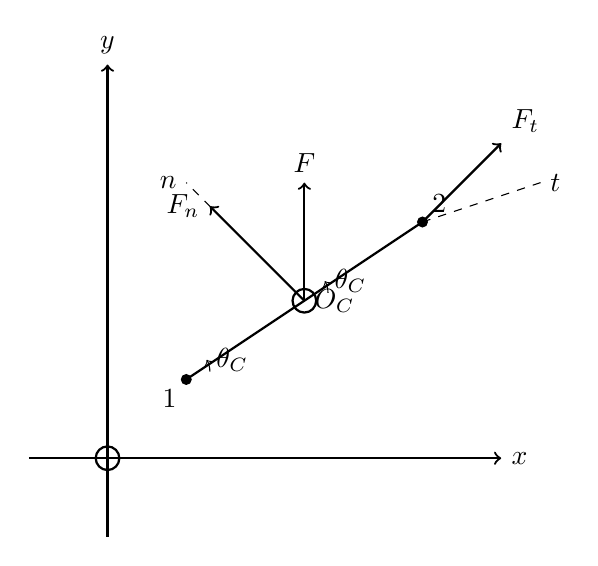
\begin{tikzpicture}
    
    % Axes
    \draw[thick,->] (-1,0) -- (5,0) node[right] {$x$};
    \draw[thick,->] (0,-1) -- (0,5) node[above] {$y$};
    \draw[thick] (0,0) circle (0.15); % Rotational point

    % Rod
    \draw[thick] (1,1) -- (4,3);
    
    % Points on the rod
    \fill (1,1) circle (0.07) node[below left] {1};
    \fill (4,3) circle (0.07) node[above right] {2};
    
    % Center of mass
    \draw[thick] (2.5,2) circle (0.15) node[right] {$O_C$};

    % Forces
    \draw[->,thick] (4,3) -- ++(1,1) node[above right] {$F_t$};
    \draw[->,thick] (2.5,2) -- ++(0,1.5) node[above] {$F$};
    \draw[->,thick] (2.5,2) -- ++(-1.2,1.2) node[left] {$F_n$};
    
    % Tangent and normal directions
    \draw[dashed] (4,3) -- ++(1.5,0.5) node[right] {$t$};
    \draw[dashed] (2.5,2) -- ++(-1.5,1.5) node[left] {$n$};

    % Angles
    \draw[->] (1,1) ++(0.3,0.1) arc (0:30:0.3) node[right] {$\theta_C$};
    \draw[->] (2.5,2) ++(0.3,0.1) arc (0:30:0.3) node[right] {$\theta_C$};
 
    \end{tikzpicture}
    \caption{Shows a rod shaped backbone of an elliptical cell made from two masses $m_1 = m_2 = m$ connected by a massless rod of length $2d$}
    \label{fig:enter-label}
\end{figure}



Add in a flow chart ??? Diagrammatic representation of the code. 









